\documentclass[11pt]{article}

\usepackage[margin=1in]{geometry}
\usepackage{amsmath,amssymb,mathtools}
\usepackage{graphicx}
\usepackage{booktabs}
\usepackage{longtable}
\usepackage{array}
\usepackage{float}
\usepackage{microtype}
\usepackage{enumitem}
\usepackage{setspace}
\usepackage{xcolor}
\usepackage{hyperref}
\usepackage{caption}

\hypersetup{
  colorlinks=true,
  linkcolor=black,
  citecolor=black,
  urlcolor=blue,
  pdftitle={The Harlequin Paradox: Strategic Absurdity in Negotiation},
  pdfauthor={Don Merrow}
}

\setstretch{1.08}

\title{\textbf{The Harlequin Paradox}\\[0.35em]
\large Strategic Absurdity in Negotiation}

\author{
Don Merrow\\
Founder, IcreateCrypto\\
Vancouver, Canada
}

\date{July 1, 2025\\Recovered and Formalized Edition}

\begin{document}

\maketitle

\begin{abstract}
Aggressive behavior in negotiation and conflict often seeks to reduce uncertainty and collapse ambiguity through dominance or threat. This paper introduces the Harlequin Paradox, a theoretical model in which humorous or absurd responses destabilize that strategy by expanding the field of informational possibilities. Rather than resisting or submitting, the humorous actor reframes the encounter and forces a renegotiation of meaning, status, and audience interpretation.

The model describes three interacting dimensions. \emph{Aggressor influence equivalence} represents perceived dominance and the social pressure supporting it. \emph{Jester presence equivalence} represents contrast and potency, including resilience and delivery. \emph{Chaos factor equivalence} represents situational randomness such as timing errors, interruptions, misfires, and narrative dissonance.

Humor functions here as signal deflection rather than avoidance. It introduces dissonance, increases status risk, and can produce recursive ambiguity under observation. A simulation demonstration is provided to show how outcomes vary with uncertainty injection, crowd amplification, shame susceptibility, endurance, and chance.

The core mathematical model is presented first. Time-integrated dynamics, exhaustion, phase-space analysis, refractive attention, factorial layouts, and Hamiltonian-style extensions are placed in appendices so that the original theory remains readable while the later mathematics remains available for scrutiny.
\end{abstract}

\section{Introduction}

In most social, political, and psychological models of conflict, aggression expects a response such as fight, flight, or submission. These reactions validate the aggressor's frame and establish a predictable interaction loop. When a target responds with humor, absurdity, nonsense, or poetic misdirection, the aggression can become ungrounded. The aggressor is forced to re-evaluate in real time, often with observers present.

The Harlequin Paradox examines this dynamic using a formal framework that tracks three dimensions: aggressor influence equivalence, jester presence equivalence, and chaos factor equivalence. The central claim is not that humor always prevails, but that it can create a new interaction surface where aggression loses efficiency, particularly when status and audience perception become unstable variables.

What began as a coping behavior at the individual level now appears on larger social and diplomatic stages. Humor reframes the interaction space not only cognitively but tactically. In some contexts, power is undone not by opposition, but by confusion.

\section{Defining the Paradox}

Let aggression represent hostile action, verbal, physical, or social. Conventional responses either counter aggression directly or yield to it, reinforcing the aggressor's framing. A humorous response does neither. It reframes the interaction by shifting the interpretive context rather than contesting force.

The humorous actor operates outside the expected response set, introducing ambiguity that disrupts prediction. This disruption can produce confusion, public loss of control, or diminished status in the aggressor. Whether the reframing succeeds depends on the relative strengths of dominance pressure versus disruption potential, and on whether the environment amplifies or dampens the reframing.

The paradox can be stated simply:

\begin{quote}
The apparently unserious move may become the most strategically serious move available.
\end{quote}

The fool looks unarmed because the weapon is not force. The weapon is frame instability.

\section{Historical Illustrations of the Paradox}

While fictional scenarios can help explain the Harlequin Paradox, real-world events offer vivid and sometimes surprising examples of humor, absurdity, play, or accidental comedy changing the rules of an encounter.

\subsection{The Christmas Truce of 1914}

British and German soldiers paused hostilities to sing songs, exchange gifts, and play football. For a short time, shared humanity interrupted the machinery of war.

\subsection{Queen Elizabeth II and the Goon Show}

Before becoming queen, Princess Elizabeth participated in a parody associated with a famous radio comedy. The episode contributed to a more approachable public image of the monarchy.

\subsection{Ping-Pong Diplomacy}

Informal contact between American and Chinese table-tennis players helped create an opening for renewed diplomatic communication after years of separation.

\subsection{Apollo--Soyuz}

During the Cold War, American astronauts and Soviet cosmonauts met in orbit, exchanged handshakes, and shared a public moment of human cooperation.

\subsection{Satire and the Velvet Revolution}

Absurd theater, parody, and public mockery helped weaken the emotional authority of rigid political power in Czechoslovakia.

These cases are illustrations rather than controlled proofs. They show the recurring structure of the paradox: surprise, contrast, and play can interrupt established roles and open a path that direct opposition may not create.

Laughter, when used well, does not retreat. It is a tool of gentle rebellion.

\section{Silly Equilibrium: How Humor Shifts the Game}

Define the following variables as a compact simulation scaffold.

\begin{longtable}{>{\raggedright\arraybackslash}p{0.18\textwidth}
                  >{\raggedright\arraybackslash}p{0.72\textwidth}}
\toprule
\textbf{Symbol} & \textbf{Meaning}\\
\midrule
\endhead

$A$ & Aggressor.\\
$T$ & Target or potential Silly Fighter.\\
$S$ & Stance rigidity of the target or interaction. A held stance is confrontational; a loose stance is adaptive, playful, or evasive.\\
$L$ & Level of aggression, often normalized to $[0,1]$.\\
$R$ & Response type, such as normal response, humor, or humor plus escape.\\
$P_{\mathrm{aggr}}$ & Perceived dominance of the aggressor.\\
$U$ & Uncertainty introduced into the interaction.\\
$E$ & Emotional shift in the aggressor, including laughter, confusion, anger, or shame.\\
$C$ & Crowd engagement level.\\
$C_{\mathrm{size}}$ & Crowd size or audience scale.\\
$T_{\mathrm{pain}}$ & Jester pain threshold or endurance under sustained pressure.\\
$S_{\mathrm{aggr}}$ & Shame susceptibility of the aggressor.\\
$A_{\mathrm{size}}$ & Aggressor physical, social, or institutional scale.\\
$J_{\mathrm{size}}$ & Jester physical or social scale, including comic contrast.\\
$H_{\mathrm{effect}}$ & Humor effectiveness, influenced by delivery, timing, context, age, and contrast.\\
$X$ & Chaos variable representing interference, misfires, accidents, and disruptive chance events.\\

\bottomrule
\end{longtable}

\subsection{Aggregated Influence Terms}

Define aggressor influence equivalence as

\begin{equation}
\Phi_A
=
P_{\mathrm{aggr}}
L
S
A_{\mathrm{size}}.
\label{eq:phi-a}
\end{equation}

Define jester presence equivalence as

\begin{equation}
\Phi_J
=
U(H_{\mathrm{effect}})
+
T_{\mathrm{pain}}
+
C\,C_{\mathrm{size}}\,S_{\mathrm{aggr}}\,J_{\mathrm{size}}
+
X.
\label{eq:phi-j}
\end{equation}

Here, $U(H_{\mathrm{effect}})$ denotes uncertainty produced through effective humor. In the simulation code, this may be implemented as either a generic function or the simpler product

\begin{equation}
U(H_{\mathrm{effect}})
=
U\,H_{\mathrm{effect}}.
\label{eq:u-h-product}
\end{equation}

The choice must be stated explicitly in any implementation.

\subsection{The Silly Equilibrium Condition}

Let Silly Equilibrium, denoted $SE$, hold when

\begin{equation}
\Phi_A < \Phi_J.
\label{eq:se-compact}
\end{equation}

Expanded,

\begin{equation}
P_{\mathrm{aggr}}LSA_{\mathrm{size}}
<
U(H_{\mathrm{effect}})
+
T_{\mathrm{pain}}
+
C\,C_{\mathrm{size}}\,S_{\mathrm{aggr}}\,J_{\mathrm{size}}
+
X.
\label{eq:se-expanded}
\end{equation}

Define the Harlequin margin

\begin{equation}
\Delta\Phi
=
\Phi_J-\Phi_A.
\label{eq:delta-phi}
\end{equation}

Then

\begin{equation}
SE
\quad\Longleftrightarrow\quad
\Delta\Phi>0.
\label{eq:se-margin}
\end{equation}

This means that the force of aggression has become weaker than the combined influence of uncertainty, endurance, social amplification, comic dissonance, and chaos.

\subsection{Emotional Destabilization}

Define emotional destabilization of the aggressor as

\begin{equation}
E_{\mathrm{aggr}}
=
f\!\left(
H_{\mathrm{effect}},
C,
L,
T_{\mathrm{pain}},
S_{\mathrm{aggr}},
J_{\mathrm{size}},
X
\right).
\label{eq:e-aggr}
\end{equation}

The remaining control margin is

\begin{equation}
M_{\mathrm{control}}
=
P_{\mathrm{aggr}}-E_{\mathrm{aggr}}.
\label{eq:control-margin}
\end{equation}

A local disruption occurs when

\begin{equation}
M_{\mathrm{control}}<\theta_E,
\label{eq:success-threshold}
\end{equation}

where $\theta_E$ is a context-dependent threshold.

In plain terms: when emotional surprise outweighs expected control, aggression can fail.

\subsection{What Humor Adds}

\begin{itemize}
\item \textbf{Uncertainty}: destabilizes expected dominance.
\item \textbf{Emotional disruption}: evokes laughter, confusion, hesitation, anger, or shame.
\item \textbf{Crowd amplification}: increases the social consequence of losing control.
\item \textbf{Durability}: allows the jester to continue without immediately escalating.
\item \textbf{Shame sensitivity}: makes the aggressor more responsive to public interpretation.
\item \textbf{Visual irony}: amplifies mismatch and comic contrast.
\item \textbf{Chaos}: introduces real-world novelty that neither side fully controls.
\end{itemize}

\subsection{Conditions That Strengthen the Effect}

The effect may strengthen through:

\begin{itemize}
\item larger or more attentive crowds;
\item a loose, playful stance;
\item fast and relevant jokes;
\item a durable jester;
\item strong visual or social contrast;
\item empathetic reframing;
\item unusual timing, accidents, or outside interference.
\end{itemize}

The Silly Equilibrium is a tipping point, not a surrender. It shows that strength is not always louder. Sometimes it is weirder, funnier, and more surprising.

In a system designed for force, absurdity becomes a counterforce: a juggler in a world of spears.

\section{Implications and Applications}

\subsection{Social Justice and Protest}

Absurdity is not necessarily weak. It can be strategic. Clowning, parody, theatrical signage, costume, and playful refusal may disrupt authoritarian presentation by shifting attention away from fear and toward contradiction.

In this model, laughter creates psychic static. The aggressor's perceived strength fades when power becomes the punchline. This shift is emotional, not physical.

The ethical aim is not humiliation for its own sake. It is the creation of an alternative frame in which domination becomes harder to sustain.

\subsection{AI Design and Emotional Interfaces}

Artificial intelligence may be capable of defusing arguments not only through logic, but through bounded humor, ironic empathy, playful reframing, and non-reactive endurance.

A Harlequin-capable agent would require:

\begin{itemize}
\item sensitivity to danger and escalation;
\item explicit limits on mockery;
\item context-aware comic timing;
\item non-repetitive responses;
\item tolerance for insult without retaliation;
\item a measurable objective of reducing distance to resolution.
\end{itemize}

The goal is not to make machines flippant. It is to allow them to shift tension rather than merely argue or submit.

\subsection{Education and Conflict Mediation}

Children and communities are often presented with only two choices: fight back or give in. Emotional redirection offers a third path.

The core idea is not to provoke or humiliate, but to neutralize. Surprise and empathy can reframe aggression as something off-script or unstable.

Through that lens, the jester is not a fool. The jester is a teacher of emotional redirection.

\section{Limitations and Ethical Considerations}

Humor is powerful, but it is also dangerous when misunderstood.

It is culturally specific. What one group finds funny, another may see as offensive or threatening. Misfired humor can escalate conflict. A joke meant to disarm may be received as mockery. When dealing with people highly sensitive to shame, humor may feel like a trap rather than relief.

This strategy also assumes some level of safety. In a truly violent situation, playful reframing may not protect the target. Emotional resilience must never be used as an excuse to keep someone in harm's way.

The jester's appearance, clothing, body language, age, tone, and social role may strengthen or weaken the effect depending on context.

The Harlequin Paradox is not a license to ridicule. It is a call to transform conflict, not intensify it. Its greatest strength is in creating humility, not dominance.

\section{Conclusion}

The Harlequin Paradox shows that aggression can sometimes be dissolved, not merely resisted, through unexpected emotional intelligence.

Laughter, when delivered with skill, reframes power. Absurdity becomes not escape, but engagement through different terms.

In spaces of tension, unpredictability becomes armor. Humor becomes both signal and shield. When emotional resilience, surprise, and social amplification align, the target may do more than survive aggression; the target may unravel its organizing frame.

This is not theory for jesters only. It is for diplomats, educators, programmers, mediators, and anyone navigating conflict in a world of hard edges.

Strategic absurdity is not an escape from pain. It is a transformation of how pain behaves.

Control does not always come from strength. Sometimes it comes from surprise, joy, and the quiet chaos of well-timed laughter.

\section{Contextual Foundations}

The Harlequin Paradox is presented as an original synthesis, but its spirit echoes through prior work in philosophy, psychology, literature, social theory, and performance.

\subsection{Epictetus}

Stoic self-mastery emphasizes control over one's own response rather than control over the world. The jester's stance is stoicism with a grin.

\subsection{John Nash}

Nash equilibrium provides a language for strategic interaction. The Harlequin model differs because it emphasizes disruption of the response space rather than stable strategic parity.

\subsection{Harlan Ellison}

\emph{``Repent, Harlequin!'' Said the Ticktockman} presents absurdity as resistance against rigid systems.

\subsection{Erving Goffman}

Frame analysis helps explain how social encounters depend on shared interpretations. Humor can force a frame shift.

\subsection{Douglas Hofstadter}

Recursion, paradox, and play show how systems can reflect upon and destabilize themselves.

\subsection{Mikhail Bakhtin}

The carnivalesque demonstrates how parody and grotesque inversion can temporarily reverse hierarchy.

\subsection{Chaos Theory}

Small, unpredictable changes can produce disproportionately large differences in outcome. The variable $X$ represents this sensitivity to interruption and chance.

These are not technical dependencies. They are tuning forks. They help us recognize the paradox as both ancient and newly formalized.

If it has been described before, it has not been assembled here in this form.

So I name it now.

This paradox is not silly. It is not stupid. It is the evolution of negotiation:

\begin{quote}
Be funny, and you might just win.
\end{quote}

\section{Simulation Data and Model}

The original computational demonstration sampled $N=1000$ randomized scenarios.

For trial $i$, define

\begin{equation}
\Phi_A^{(i)}
=
P_{\mathrm{aggr}}^{(i)}
L^{(i)}
S^{(i)}
A_{\mathrm{size}}^{(i)},
\end{equation}

and

\begin{equation}
\Phi_J^{(i)}
=
U^{(i)}H_{\mathrm{effect}}^{(i)}
+
T_{\mathrm{pain}}^{(i)}
+
C^{(i)}
C_{\mathrm{size}}^{(i)}
S_{\mathrm{aggr}}^{(i)}
J_{\mathrm{size}}^{(i)}
+
X^{(i)}.
\end{equation}

Then

\begin{equation}
\Delta\Phi^{(i)}
=
\Phi_J^{(i)}-\Phi_A^{(i)}.
\end{equation}

The simulated outcome is classified as

\begin{equation}
SE_i=
\begin{cases}
1, & \Delta\Phi^{(i)}>0,\\
0, & \Delta\Phi^{(i)}\leq 0.
\end{cases}
\end{equation}

The percentage of jester-favoured outcomes is therefore

\begin{equation}
\widehat{p}_{SE}
=
\frac{1}{N}
\sum_{i=1}^{N}
SE_i.
\label{eq:estimated-se-rate}
\end{equation}

Any percentage reported by the simulation is conditional on the selected distributions, weights, and random seed. It is not an empirical estimate of real-world success.

\subsection{Graphical Summary}

The reconstructed repository includes:

\begin{itemize}
\item a cumulative probability curve;
\item separate jester-win and aggressor-win scatter plots;
\item a combined outcome scatter plot;
\item a wave comparison over indexed Monte Carlo trials;
\item time-integrated dynamics;
\item cumulative margin;
\item outcome distributions;
\item phase-space analysis;
\item least-time refraction and least-action illustrations.
\end{itemize}

\begin{figure}[H]
\centering
\IfFileExists{figures/cumulative_probability.png}{
  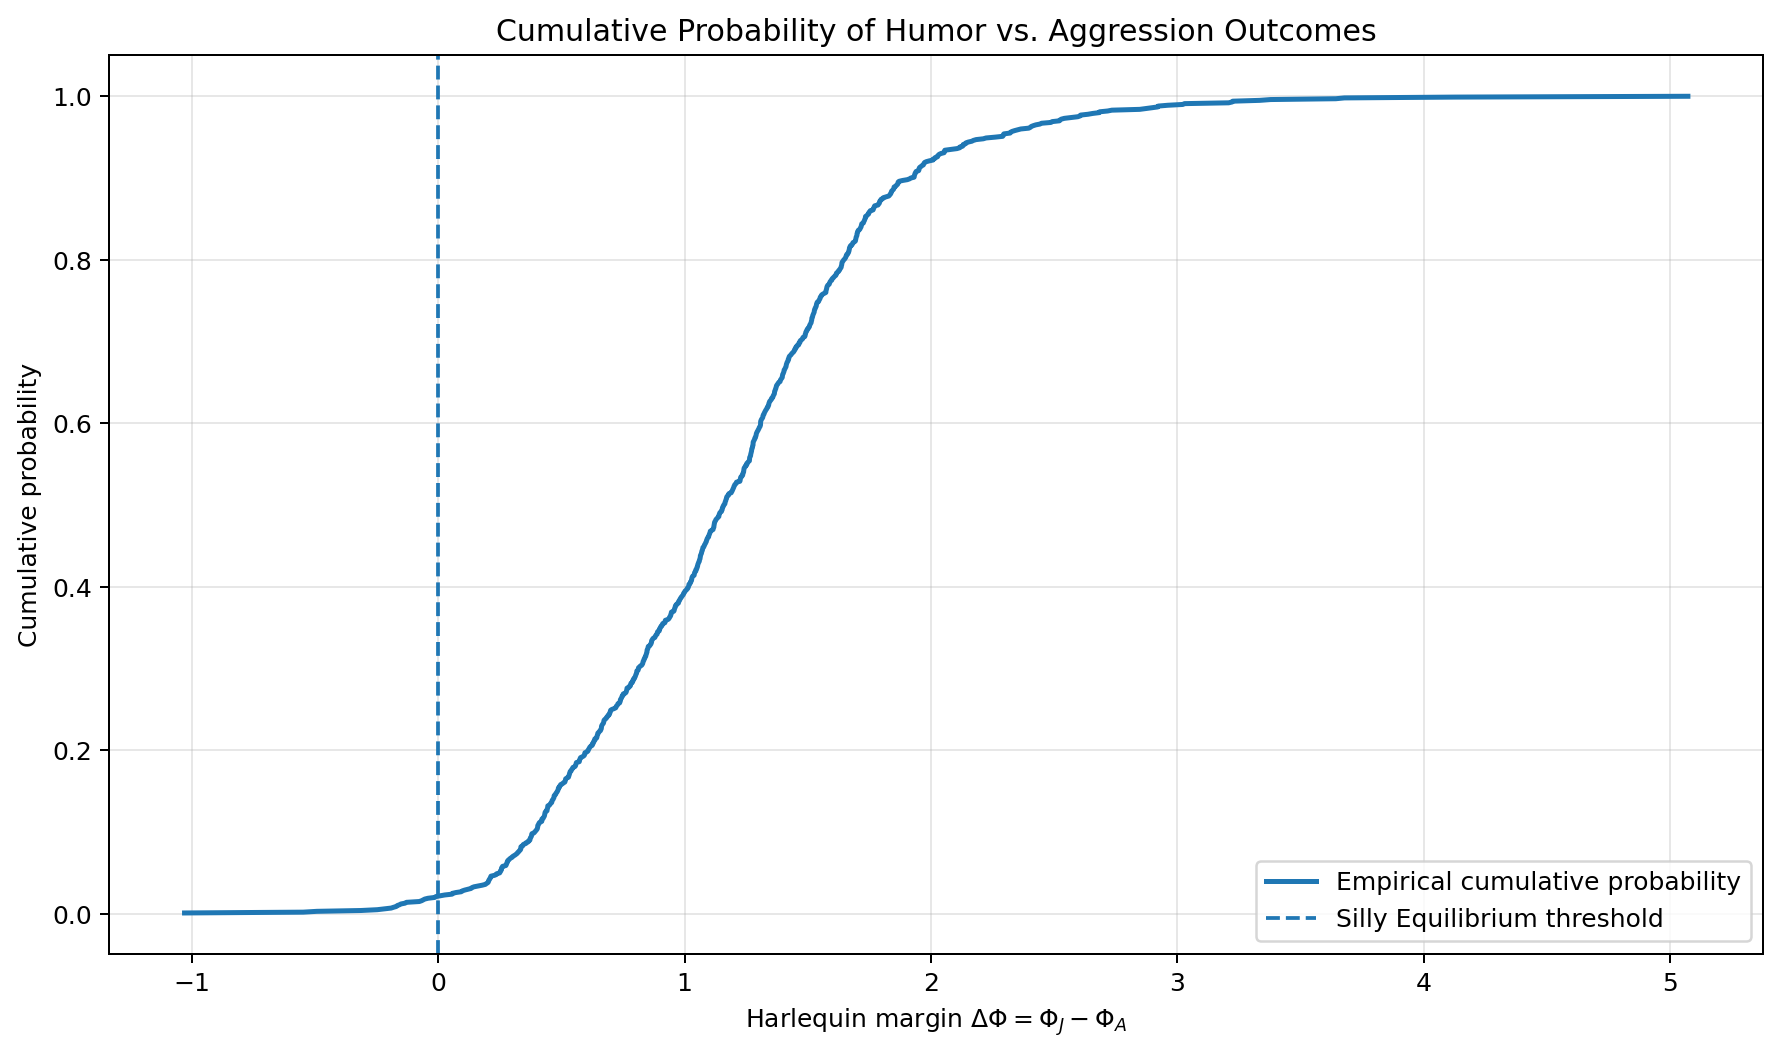
\includegraphics[width=0.92\textwidth]{figures/cumulative_probability.png}
}{
  \fbox{\parbox{0.85\textwidth}{Missing figure: \texttt{figures/cumulative\_probability.png}}}
}
\caption{Empirical cumulative distribution of the Harlequin margin.}
\end{figure}

\begin{figure}[H]
\centering
\IfFileExists{figures/combined_outcomes_scatter.png}{
  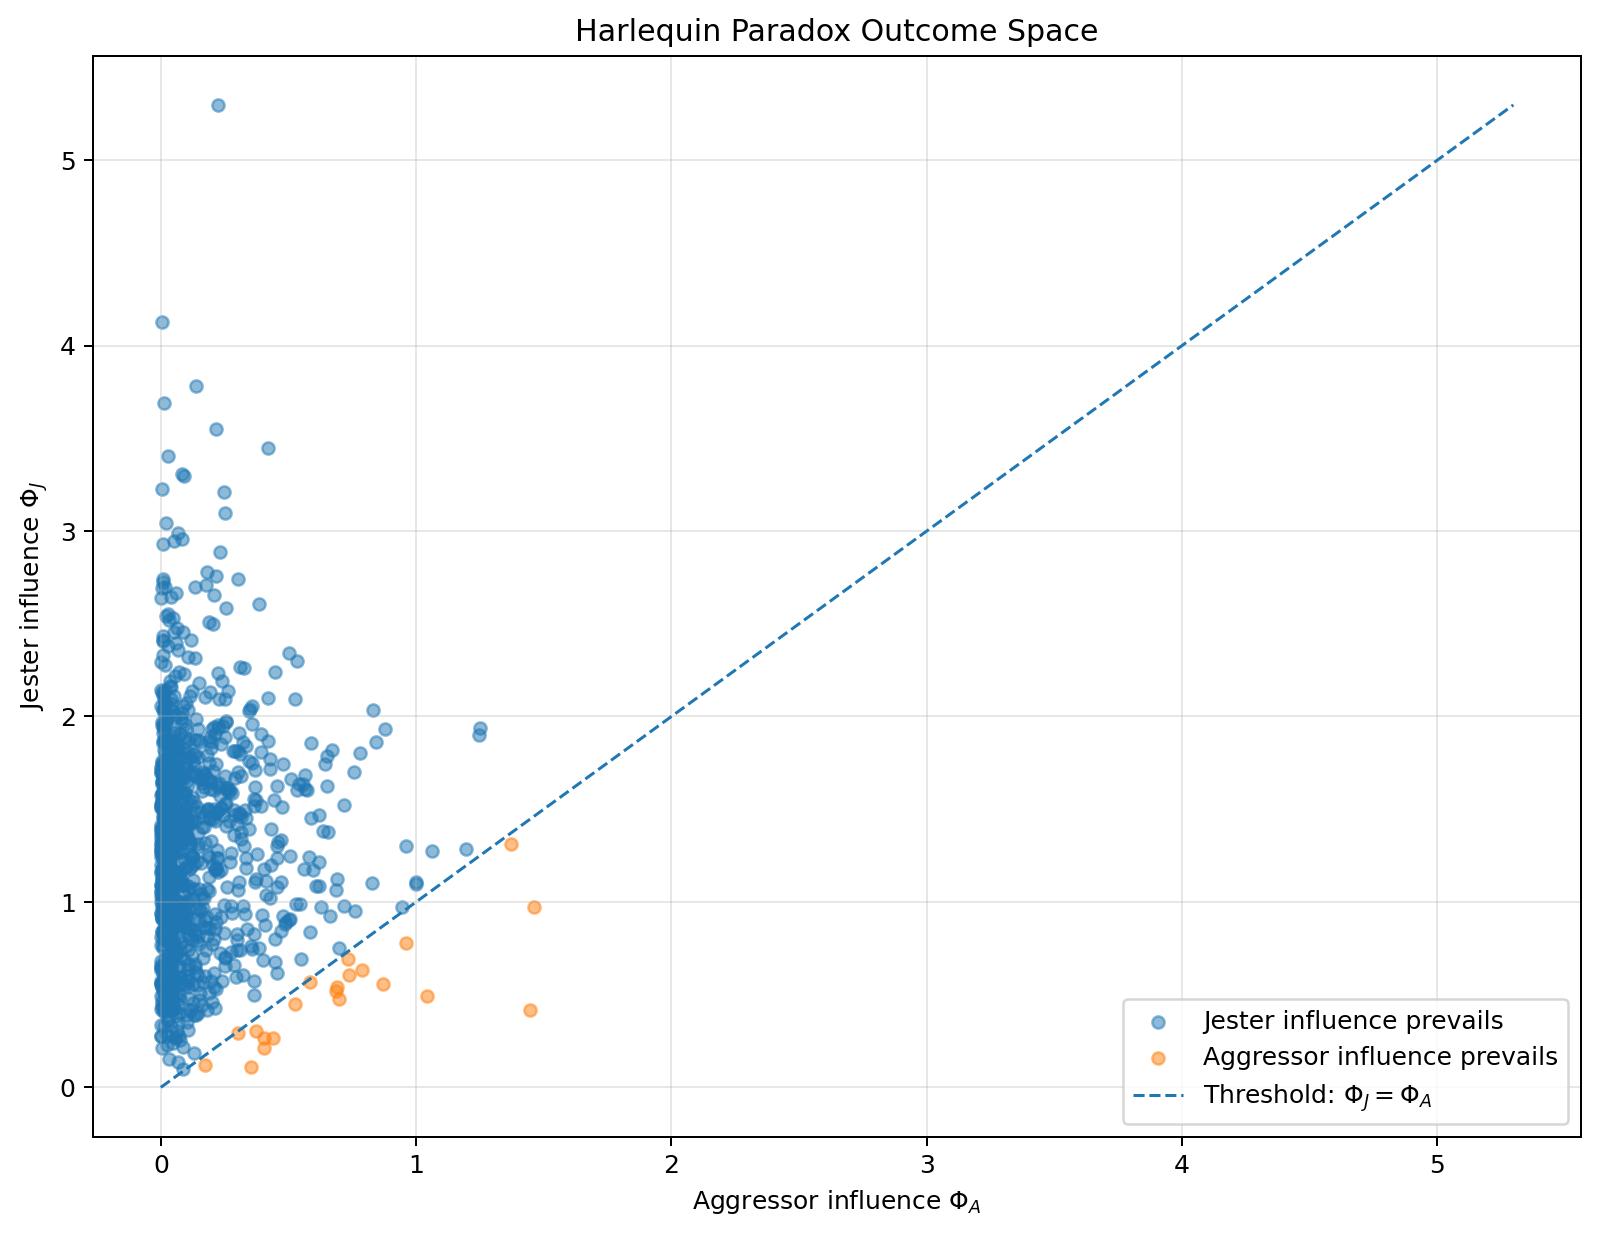
\includegraphics[width=0.92\textwidth]{figures/combined_outcomes_scatter.png}
}{
  \fbox{\parbox{0.85\textwidth}{Missing figure: \texttt{figures/combined\_outcomes\_scatter.png}}}
}
\caption{Combined simulated outcome space.}
\end{figure}

\begin{figure}[H]
\centering
\IfFileExists{figures/wave_comparison.png}{
  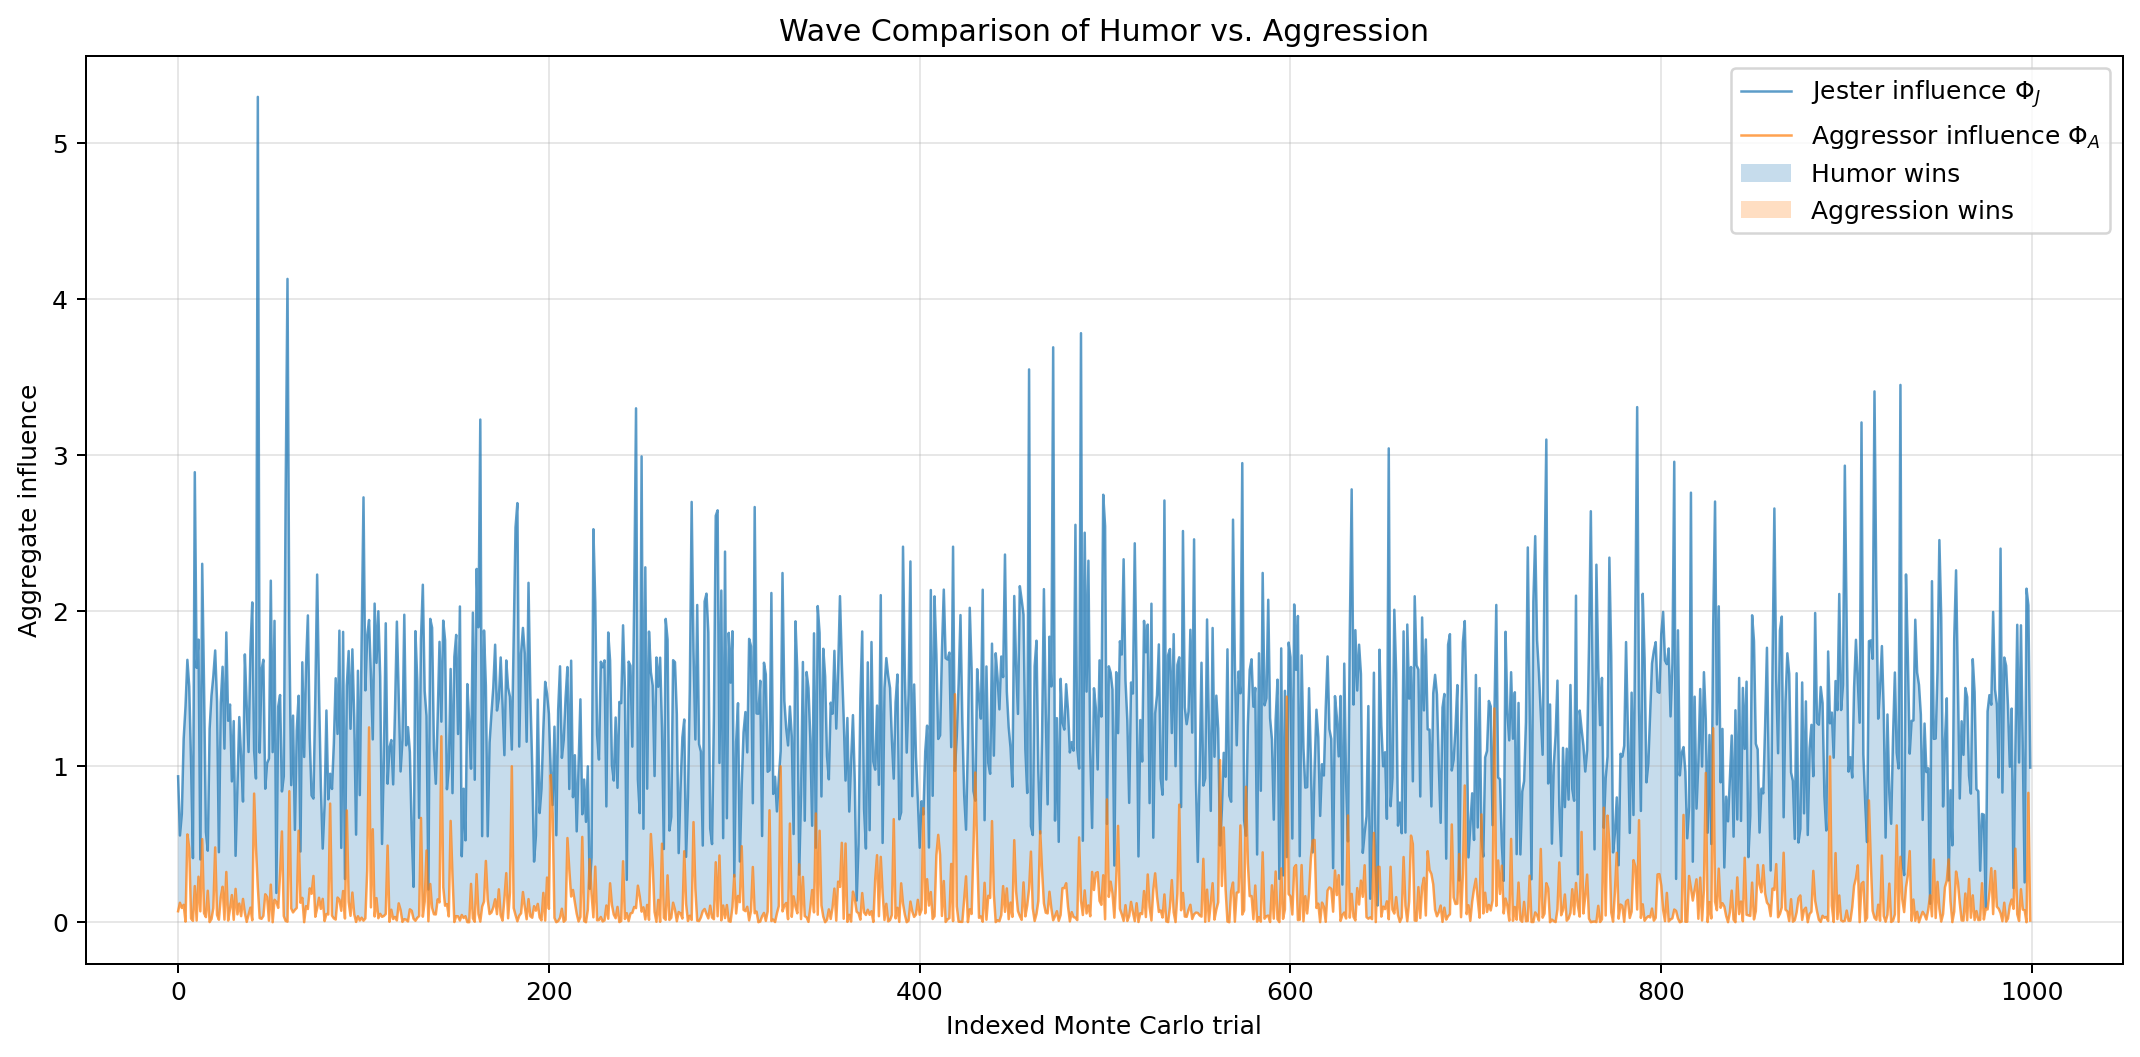
\includegraphics[width=0.92\textwidth]{figures/wave_comparison.png}
}{
  \fbox{\parbox{0.85\textwidth}{Missing figure: \texttt{figures/wave\_comparison.png}}}
}
\caption{Indexed comparison of jester and aggressor influence. The horizontal axis represents trial index, not physical time.}
\end{figure}

This is not a joke. It is how jokes win.

\appendix

\section{Exploratory Extensions and Alternative Framings}

This appendix presents later extensions that are not required for understanding the core model. They are included to preserve intellectual continuity and to invite further refinement.

\subsection{Compact Formal Field Terms}

The original field terms are

\begin{align}
\Phi_A(t)
&=
P_{\mathrm{aggr}}(t)
L(t)
S(t)
A_{\mathrm{size}},
\\
\Phi_J(t)
&=
U\!\left(H_{\mathrm{effect}}(t)\right)
+
T_{\mathrm{pain}}(t)
+
C(t)C_{\mathrm{size}}S_{\mathrm{aggr}}(t)J_{\mathrm{size}}
+
X(t).
\end{align}

The instantaneous margin is

\begin{equation}
\Delta\Phi(t)=\Phi_J(t)-\Phi_A(t).
\end{equation}

\subsection{Time-Integrated Silly Equilibrium}

Define cumulative advantage over $[0,T]$ as

\begin{equation}
D(T)
=
\int_0^T
\left[
\Phi_J(t)-\Phi_A(t)
\right]dt.
\label{eq:integrated-margin}
\end{equation}

Then a cumulative Harlequin advantage exists when

\begin{equation}
D(T)>0.
\end{equation}

The distinction is simple:

\begin{itemize}
\item $\Delta\Phi(t)$ is the instant gap;
\item $D(T)$ is the running total.
\end{itemize}

\begin{figure}[H]
\centering
\IfFileExists{figures/time_integrated_dynamics.png}{
  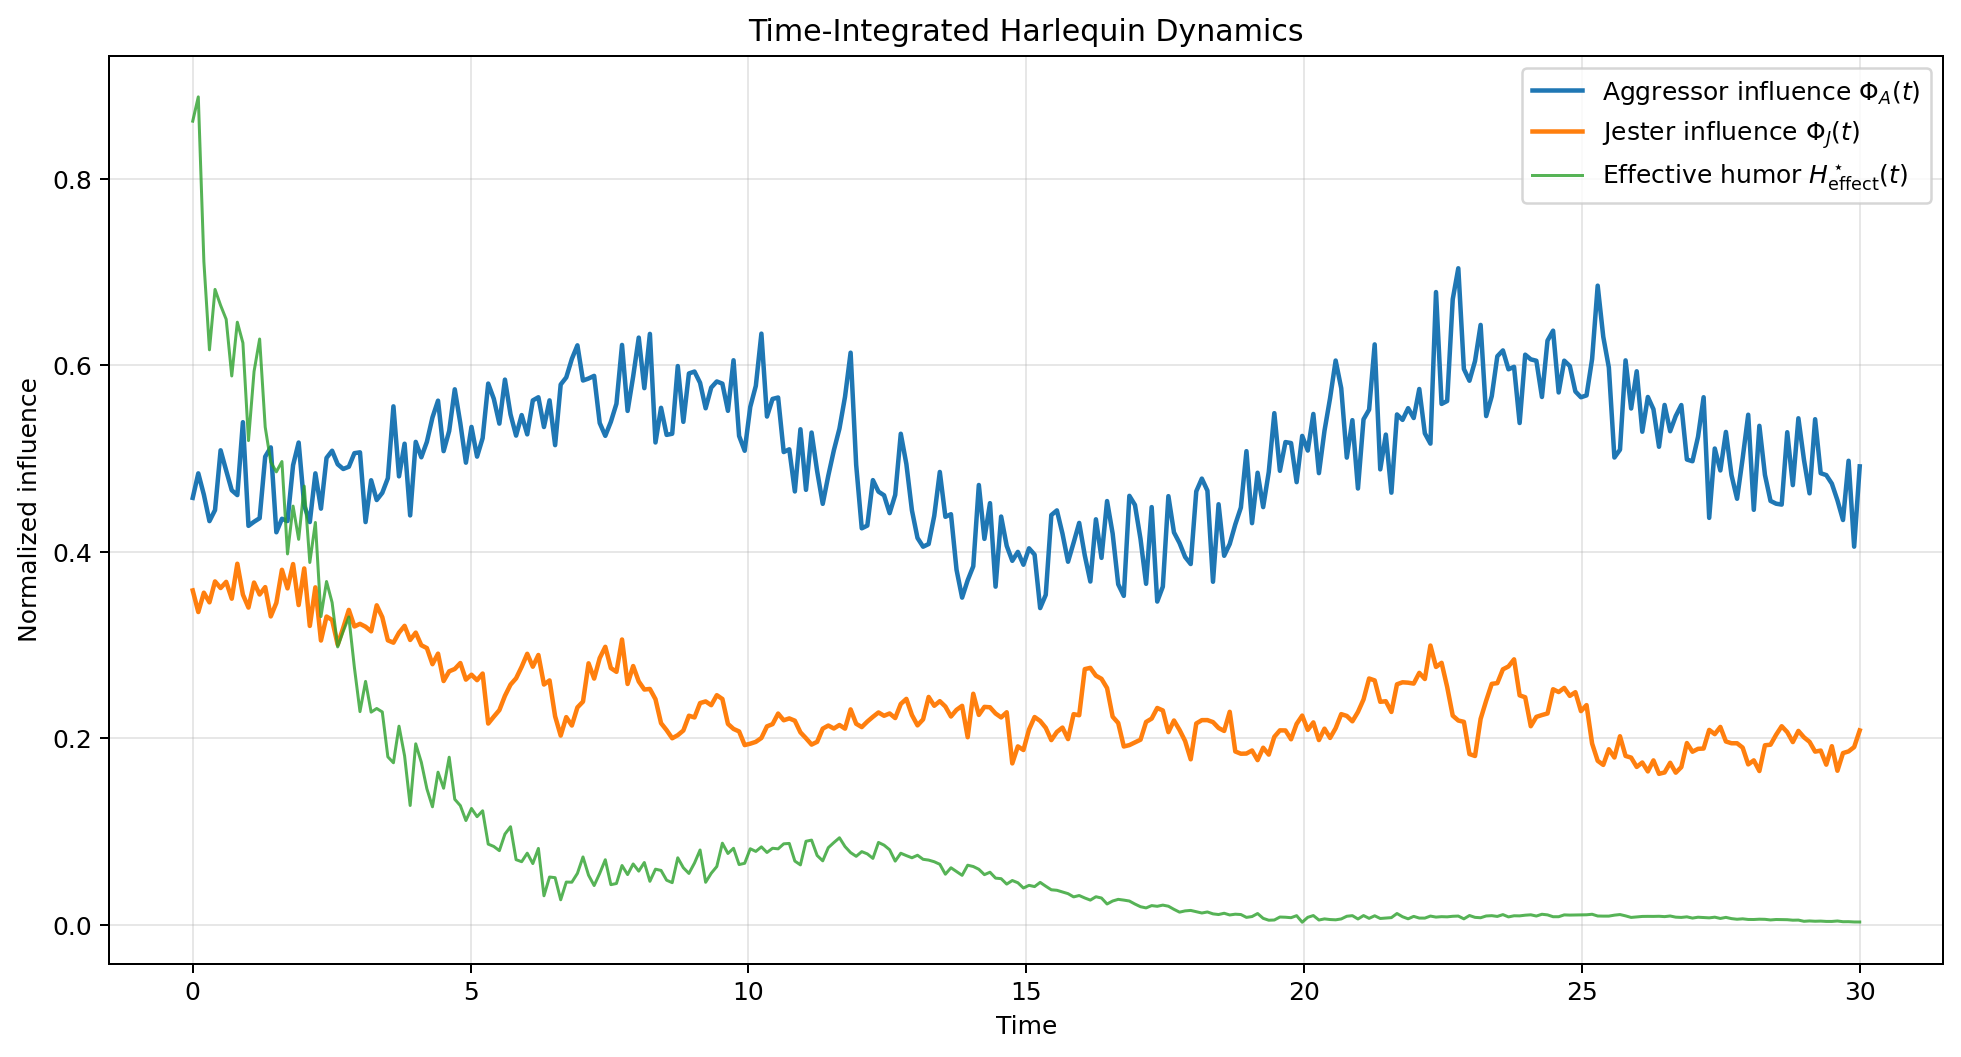
\includegraphics[width=0.92\textwidth]{figures/time_integrated_dynamics.png}
}{
  \fbox{\parbox{0.85\textwidth}{Missing figure: \texttt{figures/time\_integrated\_dynamics.png}}}
}
\caption{Time-integrated aggressor and jester influence.}
\end{figure}

\begin{figure}[H]
\centering
\IfFileExists{figures/cumulative_margin.png}{
  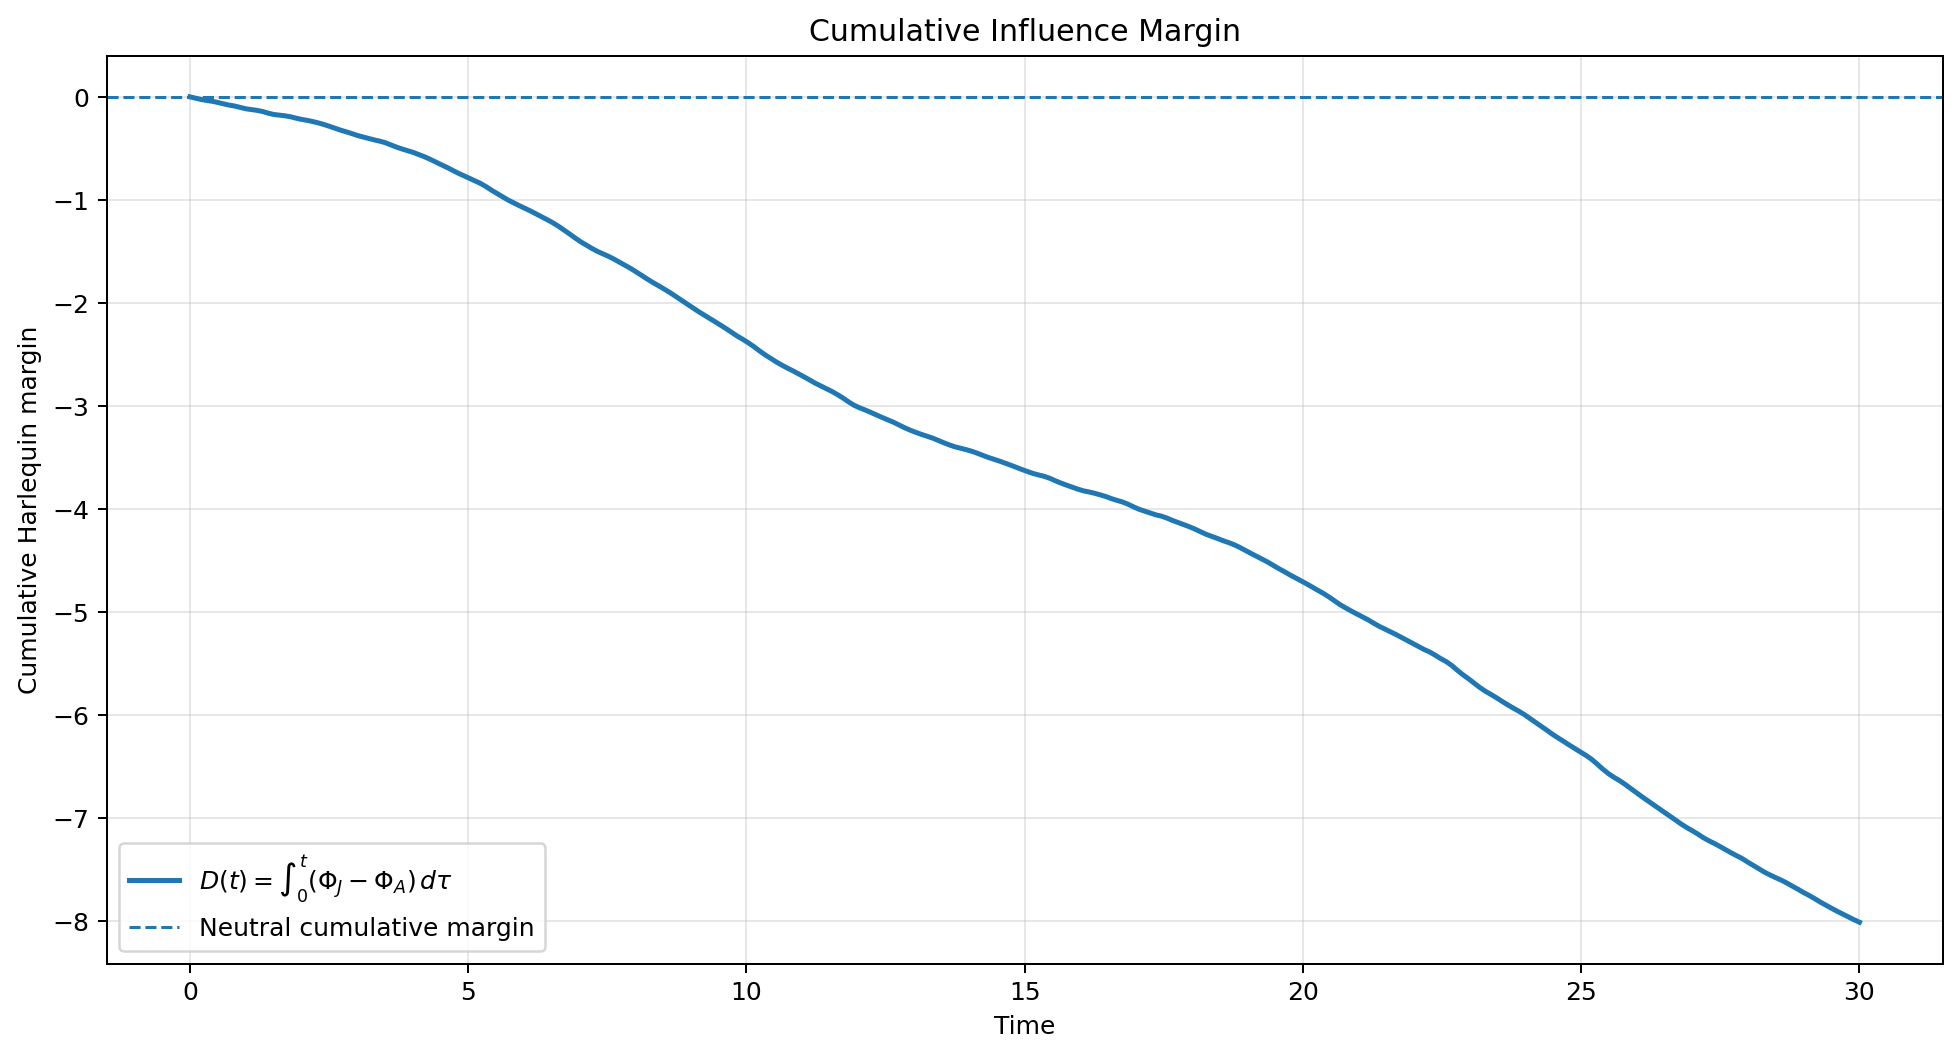
\includegraphics[width=0.92\textwidth]{figures/cumulative_margin.png}
}{
  \fbox{\parbox{0.85\textwidth}{Missing figure: \texttt{figures/cumulative\_margin.png}}}
}
\caption{Cumulative Harlequin margin.}
\end{figure}

\subsection{Harlequin Exhaustion}

Let $E_{\mathrm{exh}}(t)$ denote exhaustion. A clean evolution law is

\begin{equation}
\dot{E}_{\mathrm{exh}}
=
\alpha
\left[
w_HH_{\mathrm{effort}}(t)
+
w_A L(t)S(t)
\right]
-
\beta R_{\mathrm{rec}}(t),
\label{eq:exhaustion}
\end{equation}

subject to

\begin{equation}
E_{\mathrm{exh}}(t)\geq 0.
\end{equation}

Effective humor is damped by exhaustion:

\begin{equation}
H_{\mathrm{effect}}^\star(t)
=
H_{\mathrm{effect}}(t)
\exp\!\left[
-\kappa E_{\mathrm{exh}}(t)
\right].
\label{eq:effective-humor}
\end{equation}

\subsection{Safety Abort}

Define immediate risk

\begin{equation}
R_{\mathrm{risk}}(t)
=
L(t)A_{\mathrm{size}}.
\end{equation}

Abort the humorous strategy when

\begin{equation}
R_{\mathrm{risk}}(t)>\rho.
\end{equation}

Safety beats style.

\subsection{Distance to Resolution}

Let $q(t)$ denote the state of the unresolved issue and $q^\star$ an acceptable resolution state. Define

\begin{equation}
d_R(t)
=
\left\|
q(t)-q^\star
\right\|.
\end{equation}

Define resolution velocity

\begin{equation}
v_R(t)
=
-\frac{d}{dt}d_R(t).
\end{equation}

Then

\begin{align}
v_R(t)&>0 &&\text{movement toward resolution},\\
v_R(t)&=0 &&\text{no meaningful closure},\\
v_R(t)&<0 &&\text{movement away from resolution}.
\end{align}

The strongest outcome is

\begin{equation}
\Phi_J>\Phi_A
\quad\text{and}\quad
v_R>0.
\end{equation}

This distinguishes productive disruption from a merely performative victory.

\subsection{Delta-Based Outcome Classes}

Let

\begin{equation}
\Delta\Phi_T
=
\int_0^T
\left[
\Phi_J(t)-\Phi_A(t)
\right]dt
\end{equation}

and

\begin{equation}
\Delta d_R
=
d_R(0)-d_R(T).
\end{equation}

Then:

\begin{longtable}{p{0.22\textwidth}p{0.22\textwidth}p{0.44\textwidth}}
\toprule
\textbf{Influence} & \textbf{Resolution} & \textbf{Interpretation}\\
\midrule
\endhead

$\Delta\Phi_T>0$ & $\Delta d_R>0$ & Productive Harlequin outcome.\\
$\Delta\Phi_T>0$ & $\Delta d_R\leq 0$ & Performative victory without closure.\\
$\Delta\Phi_T\leq 0$ & $\Delta d_R>0$ & Aggressor-led closure.\\
$\Delta\Phi_T\leq 0$ & $\Delta d_R\leq 0$ & Aggressive failure or unresolved escalation.\\

\bottomrule
\end{longtable}

\subsection{Phase Space}

The phase-space plot compares playful uncertainty against aggressor influence.

Let

\begin{equation}
B
=
T_{\mathrm{pain}}
+
C\,C_{\mathrm{size}}\,S_{\mathrm{aggr}}\,J_{\mathrm{size}}
+
X.
\end{equation}

Then the decision boundary is

\begin{equation}
\Phi_A
=
U(H_{\mathrm{effect}})+B.
\end{equation}

When omitted variables are summarized by their median $\widetilde{B}$, the plotted heuristic boundary becomes

\begin{equation}
\Phi_A
=
U(H_{\mathrm{effect}})
+
\widetilde{B}.
\end{equation}

\begin{figure}[H]
\centering
\IfFileExists{figures/phase_space.png}{
  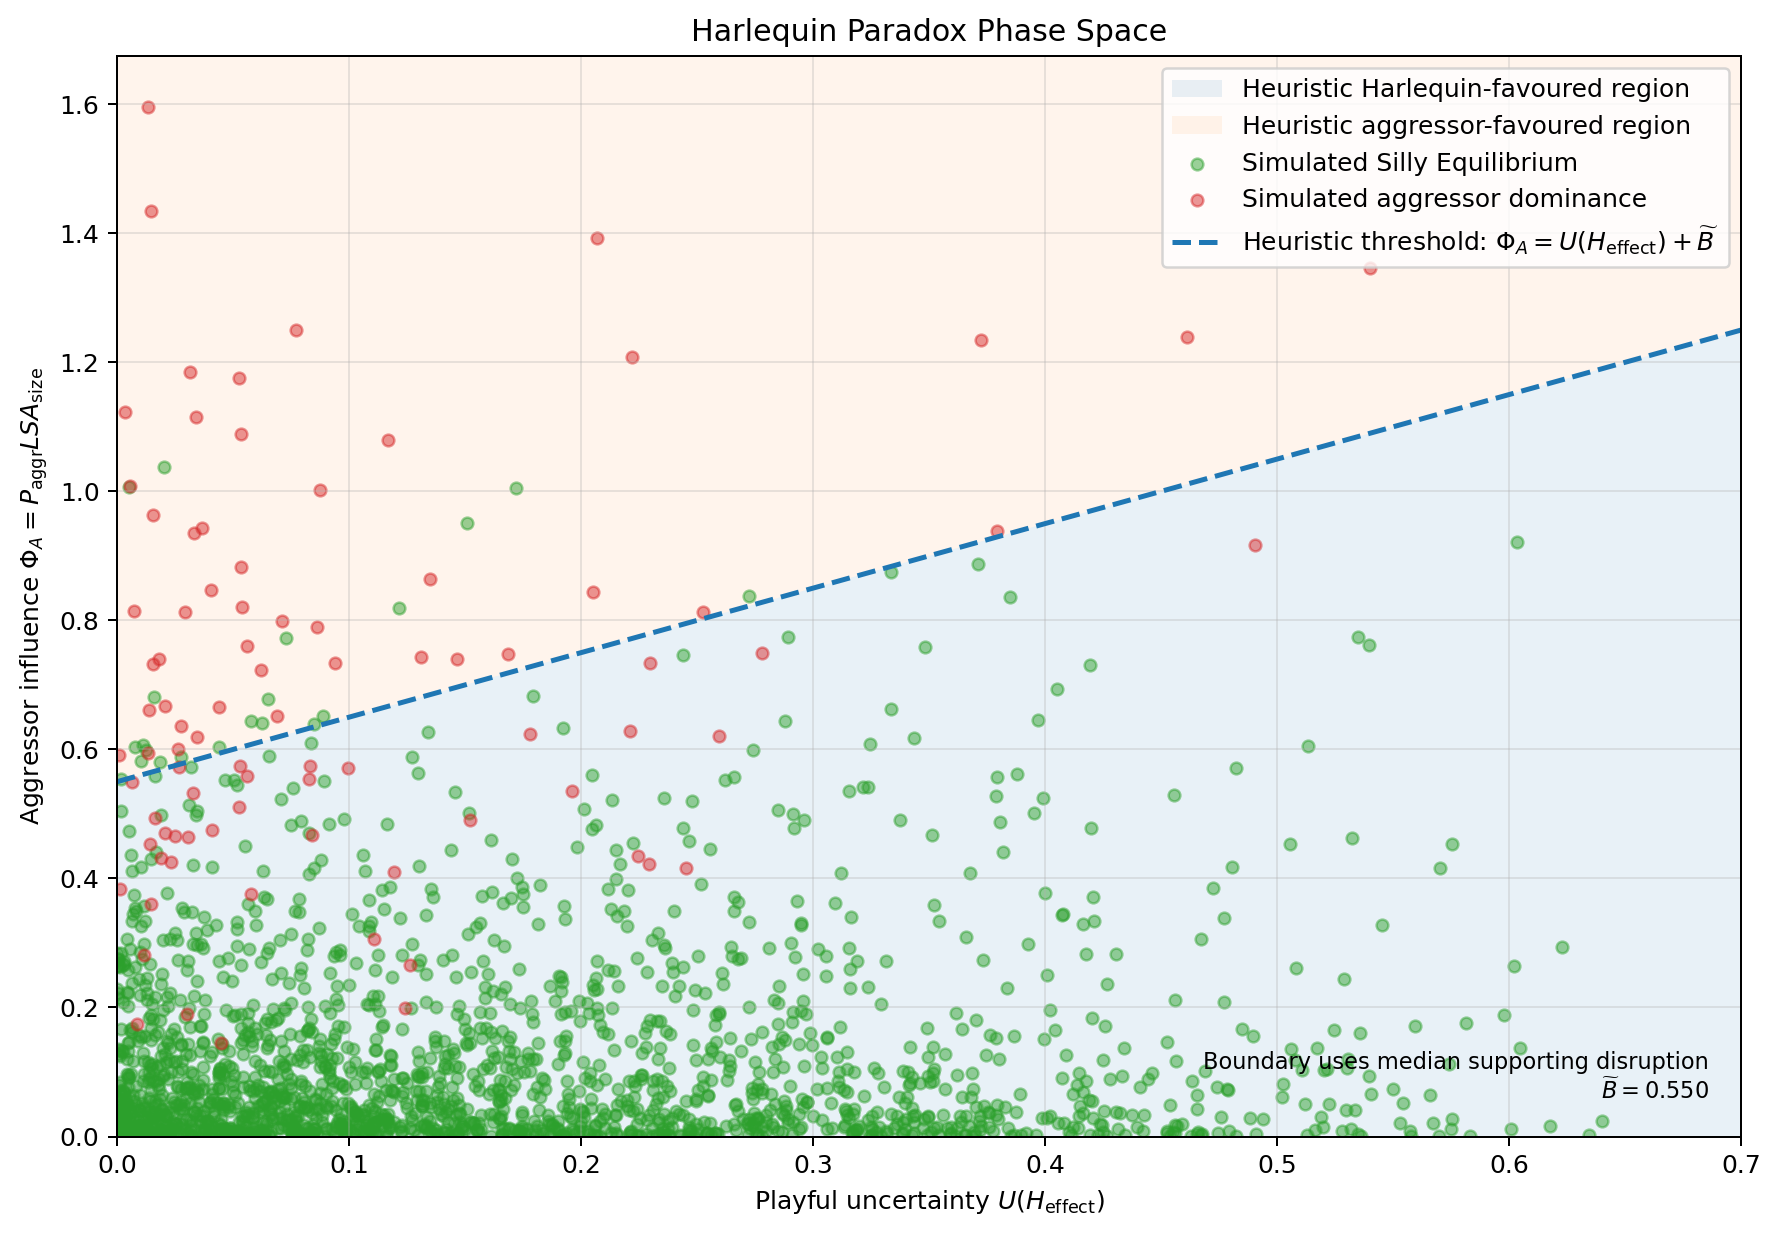
\includegraphics[width=0.92\textwidth]{figures/phase_space.png}
}{
  \fbox{\parbox{0.85\textwidth}{Missing figure: \texttt{figures/phase\_space.png}}}
}
\caption{Heuristic phase space. The displayed boundary is model-dependent, not empirical.}
\end{figure}

\subsection{Least-Time Refraction}

Map rigidity to an interpretive resistance index

\begin{equation}
n_{\mathrm{frame}}
=
n_0
+
aP_{\mathrm{aggr}}
+
bS.
\end{equation}

Map playfulness to

\begin{equation}
n_{\mathrm{play}}
=
\frac{n_1}
{1+cU(H_{\mathrm{effect}})}.
\end{equation}

Define an attention travel-time functional

\begin{equation}
T_{\mathrm{attn}}
=
\int_\Gamma
\frac{n(q)}{v_0}\,ds.
\end{equation}

Attention is modeled as bending toward the frame that becomes interpretable fastest. This is an analogy for frame selection, not a claim that attention literally obeys optics.

\begin{figure}[H]
\centering
\IfFileExists{figures/least_time_refraction.png}{
  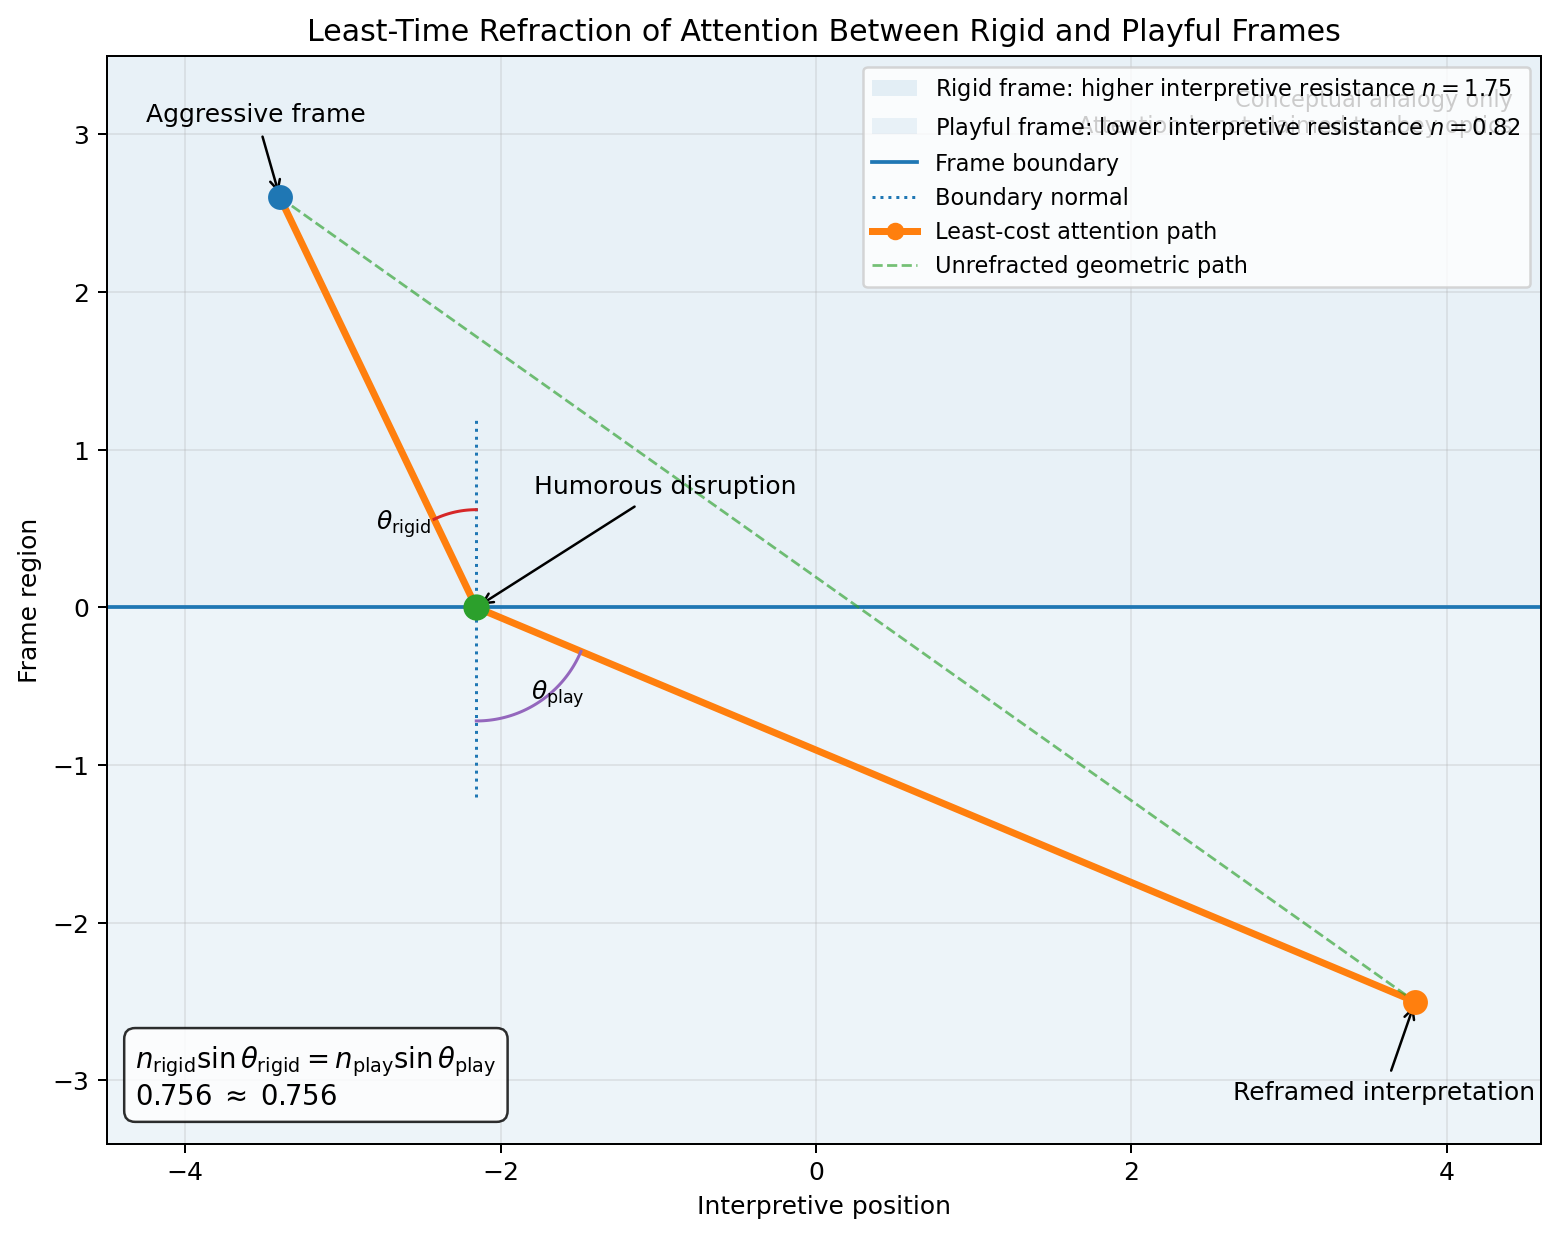
\includegraphics[width=0.88\textwidth]{figures/least_time_refraction.png}
}{
  \fbox{\parbox{0.85\textwidth}{Missing figure: \texttt{figures/least\_time\_refraction.png}}}
}
\caption{Least-time refraction analogy for attention moving between rigid and playful frames.}
\end{figure}

\subsection{Hamiltonian-Style Extension}

A Hamiltonian-style model may be used as a state-space analogy.

Let $q$ denote conflict state and $p$ interaction momentum. Define

\begin{equation}
\mathcal{H}(q,p,t)
=
K(p)
+
V(q,t)
+
V_A(q,t)
-
V_J(q,t)
+
V_{\mathrm{exh}}(t)
+
V_{\mathrm{risk}}(t).
\end{equation}

A damped stochastic evolution may be written

\begin{align}
\dot{q}
&=
\frac{\partial\mathcal{H}}{\partial p},
\\
\dot{p}
&=
-\frac{\partial\mathcal{H}}{\partial q}
-\gamma p
+\xi(t).
\end{align}

Here, $\gamma$ is damping and $\xi(t)$ is noise. The model does not claim that human behavior literally follows classical mechanics. It uses a structured energy-like accounting to compare momentum, unresolved pressure, aggression, reframing, exhaustion, and risk.

The Harlequin move does not necessarily oppose force along the same axis. It changes the field.

A perpendicular move. A tickle where others place a pawn.

\subsection{Least-Action Framing}

Define an action functional

\begin{equation}
\mathcal{S}[q]
=
\int_0^T
\mathcal{L}(q,\dot q,t)\,dt,
\end{equation}

with

\begin{equation}
\mathcal{L}
=
\frac{1}{2}m\|\dot q\|^2
-
V(q,t)
-
\lambda_A\Phi_A(t)
+
\lambda_J\Phi_J(t)
-
\lambda_EE_{\mathrm{exh}}(t)
-
\lambda_RR_{\mathrm{risk}}(t).
\end{equation}

This is a comparative model of trajectory cost, not a literal mechanical law.

\begin{figure}[H]
\centering
\IfFileExists{figures/least_action_cartoon.png}{
  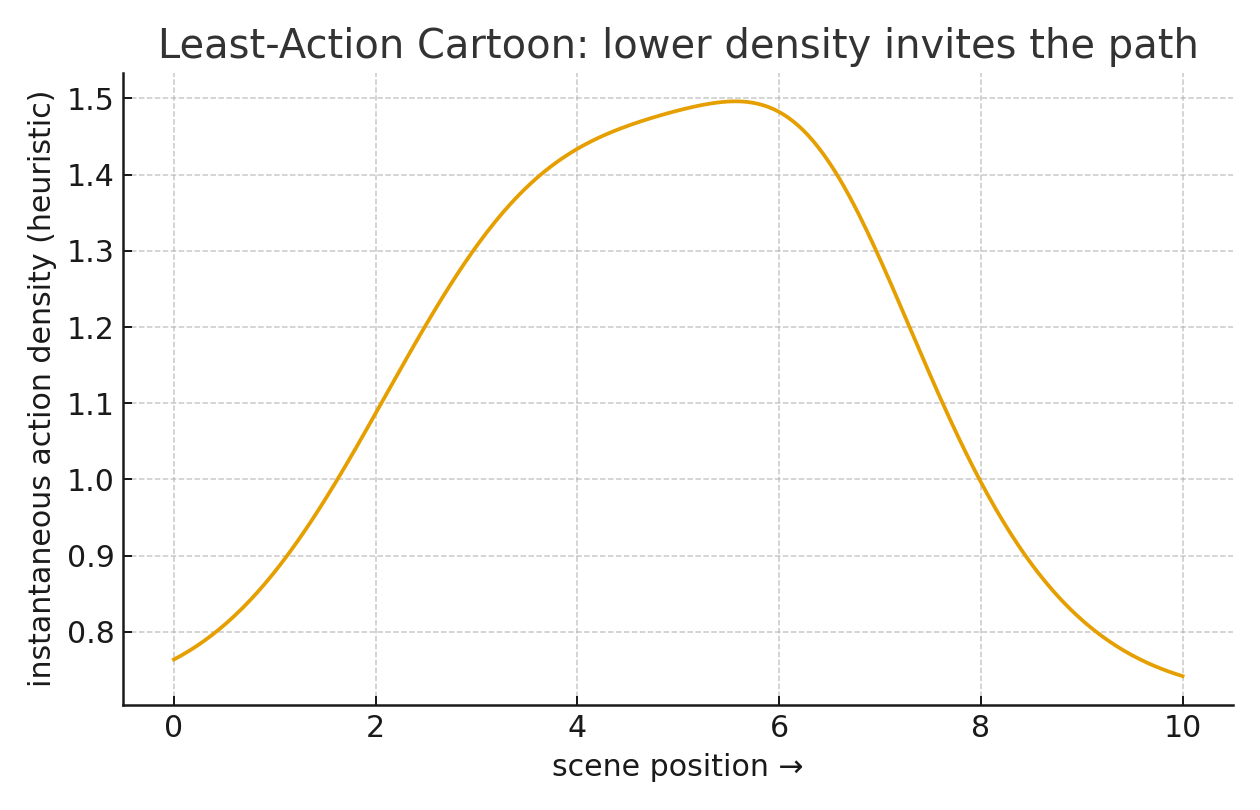
\includegraphics[width=0.88\textwidth]{figures/least_action_cartoon.png}
}{
  \fbox{\parbox{0.85\textwidth}{Missing figure: \texttt{figures/least\_action\_cartoon.png}}}
}
\caption{Conceptual comparison of conflict trajectories with different total costs.}
\end{figure}

\subsection{Factorial Interaction Layout}

A factorial design may cross:

\begin{itemize}
\item response type: quip, parody, nonsense, empathetic turn;
\item venue: private, small crowd, public;
\item audience temperature: cold, neutral, hot;
\item shame shield: low, medium, high.
\end{itemize}

A linear model may be written

\begin{equation}
Y_i
=
\mu
+
\alpha_{r(i)}
+
\beta_{v(i)}
+
\gamma_{a(i)}
+
\delta_{s(i)}
+
(\alpha\beta)_{r(i),v(i)}
+
(\alpha\gamma)_{r(i),a(i)}
+
\varepsilon_i.
\end{equation}

A mixed-effects extension may include random intercepts for aggressor, jester, culture, or repeated encounter.

\section{Editorial Note}

The Harlequin Paradox is presented in the main paper as a complete, self-contained model supported by simulation demonstrations.

The appendix is intentionally different in character. It preserves later conceptual extensions and alternative mathematical framings that emerged during development. These materials are included for transparency and future refinement, not to assert that every extension has been empirically validated.

\section{Reproducibility Note}

Each simulation should disclose:

\begin{itemize}
\item random seed;
\item sample size;
\item variable distributions;
\item weighting assumptions;
\item sign convention;
\item safety threshold;
\item software versions;
\item figure-generation commands.
\end{itemize}

Simulation percentages must not be presented as real-world empirical rates unless supported by observed and independently validated data.

\end{document}
